\documentclass[conference]{IEEEtran}
\IEEEoverridecommandlockouts
\usepackage[T1]{fontenc}
\usepackage{cite,amsmath,amssymb,booktabs,graphicx,textcomp,xcolor,balance}
\usepackage{algorithm,algorithmic}
\usepackage{tikz,pgfplots}
\usetikzlibrary{patterns,positioning,arrows.meta,shapes.misc,calc,fit}
\pgfplotsset{compat=1.16}
\usepackage[hidelinks]{hyperref}
\newcommand{\TODO}[1]{\textcolor{red}{\textbf{[#1]}}}
\newcommand{\Dr}{D_{\mathrm{reported}}}
\newcommand{\Dw}{D_{\mathrm{raw}}}
\def\BibTeX{{\rm B\kern-.05em{\sc i\kern-.025em b}\kern-.08em T\kern-.1667em\lower.7ex\hbox{E}\kern-.125em X}}
\begin{document}

\title{When Screenshot Diffing Lies: Detecting Invalid Evidence in Automated Visual Regression Testing}

\author{\IEEEauthorblockN{Tanvir Hasan}
\IEEEauthorblockA{\textit{Independent Researcher}\\
Dhaka, Bangladesh\\
tanvir.cse.cu@gmail.com}}

\maketitle

\begin{abstract}
Automated visual regression pipelines threshold a changed-pixel count between a reference and a current screenshot, and they implicitly trust that both captures, and the comparison record relating them, are valid. This assumption is rarely checked and fails silently, because a diff algorithm returns a number whether or not its inputs were meaningful. We argue that evidence validity is logically prior to differencing and belongs in a dedicated stage before thresholding. To support this view, we present a taxonomy of nine evidence-integrity failures in automated web screenshot pipelines, a lightweight and back-end-agnostic Evidence Validation Layer (EVL) that screens for them using capture metadata and image-level invariants, and an arithmetic-consistency invariant, $\Dr \le \Dw$, that flags impossible comparison records without any ground-truth defect label. In a pilot on a real capture archive of five web subjects and 81 matched capture pairs, 13.5\% of manifest entries collided on filename within a session (95\% CI 9.8--18.1\%), 11.1\% of matched pairs were invalid (6.0--19.8\%), and 4.2\% of records reaching the arithmetic gate were impossible (1.4--11.5\%), two of them attached to byte-identical captures. Re-executing the diff back-end shows that every record violating the invariant is a genuine pipeline defect (a record computed on a different session pair, or on a different page after a filename collision inside the diff tool), so the check raised no false alarm; being one-sided, it caught 5 of the 17 misattributed records. Metadata-only checks (2.6~ms/pair) missed every impossible record, whereas pixel-level checks (232~ms/pair) caught them. The pilot shows that these failures occur at non-negligible rates in a real deployment; it does not estimate their general rate.
\end{abstract}

\begin{IEEEkeywords}
visual regression testing, screenshot comparison, evidence validation, test oracle problem, flaky tests, continuous integration
\end{IEEEkeywords}

\section{Introduction}
A visual regression pipeline is mechanically simple: capture a page before a change, capture it again after, compute a difference, and decide whether the difference matters. Most effort in this space has gone into the last two steps (better diff algorithms, perceptual metrics, and thresholds); comparatively little asks whether the first two steps produced anything worth comparing.

They do not always. A screenshot can fire before a page finishes rendering, yielding a mostly blank but syntactically valid PNG; reference and current captures can depict different logical pages if a crawler's identifiers collide or drift between sessions; and a comparison tool can report a changed-pixel count that is arithmetically impossible given the two images it was handed. In an earlier pilot deployment of the same harness on a high-dynamic weather portal (18 page pairs; data in~\cite{avqrepo}), a pre-render capture at native viewport height was reported by all three diff back-ends as a 9.98--12.73\% change and ranked the third-largest regression of eighteen, although its height ratio (6.7$\times$) and file-size ratio (88$\times$) exposed it in metadata that no back-end consults. We cite this only as motivation; no result below depends on it.

The case generalizes into a question a diff algorithm cannot answer about itself: is the evidence it compares trustworthy? We call this the \emph{evidence-validity question} and argue it is distinct from, and prior to, whether a visual difference exists.

\textbf{Contributions.}
\begin{enumerate}
\item A formalization of evidence validity for screenshot-based regression testing and a taxonomy of nine evidence-integrity failures.
\item An Evidence Validation Layer (EVL) and an arithmetic-consistency invariant ($\Dr \le \Dw$) that detect invalid evidence with no seeded fault, no defect label, and no dependence on the diff back-end.
\item An evaluation on a real, in-the-wild capture archive (five subjects, 81 matched pairs) measuring capture-anomaly, invalid-pair, and impossible-record rates with confidence intervals, establishing ground truth for every impossible record by re-executing the diff back-end, and showing that metadata-only and pixel-level checks catch disjoint failures.
\end{enumerate}

\textbf{Scope of the claims.} We do not claim to be first to observe that visual tests can be unreliable (Section~\ref{sec:related}); our claim is that evidence validity can be formalized as checkable invariants that belong architecturally before differencing and thresholding. The study is a pilot: it establishes that the failures exist and are measurable, not their general prevalence. We make no claim about detection accuracy (precision or recall), because no human-verified ground truth exists for this archive, and none about the quality of any particular diff algorithm.

\section{Problem Definition}
\subsection{Terminology and the two questions}
A \emph{capture} is a screenshot plus its metadata (URL, timestamp, viewport, load time, file size, dimensions). A \emph{capture pair} $(R,C)$ associates a reference capture $R$ from an earlier session with a current capture $C$ from a later one, intended to depict the same logical page. A \emph{comparison record} is a diff back-end's output on a pair, at minimum a reported changed-pixel count $\Dr$.

The \emph{differencing question} (``how much did the page change?'') is answered by a diff algorithm on pixels, and is well defined only if $R$ and $C$ are valid evidence. The \emph{validity question} (``is this pair, and the record built from it, trustworthy enough to answer the differencing question at all?'') is answered from properties outside the pixel comparison: readability, geometric and file-size stability, timing consistent with completed rendering, correspondence to the same logical page, membership in both crawls, and arithmetic consistency of the record. A diff algorithm has no obligation to notice that its input is blank, truncated, or mispaired, so validity is logically prior to differencing. Whether a valid difference is a defect is a separate oracle question that presupposes valid evidence and is out of scope.

\subsection{Evidence-integrity failure classes}
We distinguish nine failure classes (Table~\ref{tab:taxonomy}, Section~\ref{sec:framework}): properties of a single capture (missing/unreadable, truncated, unstable geometry, file-size anomaly, abnormal metadata); properties of a pair or corpus (mismatched pairing, colliding filenames, missing corpus membership); and one property of the comparison record itself (arithmetically impossible diff). The last requires no notion of application ``ground truth'' at all, only that a comparison algorithm's arithmetic be internally consistent with the pixels it consumed.

\subsection{The arithmetic-consistency invariant}
Let $R$ and $C$ have passed geometry, file-integrity, and pair-correspondence validation. Let $W=\min(w_R,w_C)$ and $H=\min(h_R,h_C)$. We align them by cropping both to their common top-left $W\times H$ region (when the dimensions are equal, nothing is cropped), and compare pixels at identical coordinates, giving $N=W\!\cdot\!H$ aligned pixels. The diff back-end crops in the same way. Define the raw pixel-inequality count
\begin{equation}
\Dw = \bigl|\{\, i \in \{1,\dots,N\} : R_i \neq C_i \,\}\bigr|,
\end{equation}
where $R_i \neq C_i$ holds if any of the three RGB channels of pixel $i$ differs, with zero tolerance (the screenshots are opaque, so alpha is not compared). In the pilot, 71 of the 72 pairs that reach the arithmetic gate have identical dimensions; the remaining one differs in height by 1.0\% and is cropped. $\Dw$ is computed independently of any back-end. A back-end may legitimately report $\Dr < \Dw$ (anti-aliasing tolerance, perceptual weighting, and masking can only suppress change), but it cannot legitimately report
\begin{equation}
\Dr > \Dw,
\end{equation}
because no pixel can be ``more different'' than unequal. Such a record is not a disagreement about severity; it is arithmetically impossible and indicates a defect in the comparison pipeline itself (an alignment bug, a stale cached record, or an undetected corpus mismatch). It is the only EVL check that certifies invalidity purely from internal consistency, without appeal to what the page ``should'' look like, and is our strongest single contribution. It is sound but one-sided: a record that describes the wrong pair yet reports \emph{fewer} changed pixels than the pair it is attached to passes undetected (Section~\ref{sec:root}).

\section{Related Work}\label{sec:related}
\textit{Test oracles and flakiness.} Barr et al. survey the oracle problem~\cite{barr2015}; visual thresholds are a derived oracle over pixel differences, and we ask the narrower, prior question of whether that oracle's inputs are valid. Flaky-test studies~\cite{parry2022,romano2021}, including web visual flakiness~\cite{pei2026}, treat instability as a property of outcomes across repeated runs; an evidence validator instead flags an untrustworthy capture from a single session.

\textit{Cross-browser and visual testing.} WebDiff~\cite{webdiff}, X-PERT~\cite{xpert}, ReDeCheck~\cite{redecheck}, and vision-based presentation-failure localization~\cite{mahajan2015} compare configurations of one page version; we study capture reliability across time for one configuration. Work on migrating~\cite{pesto}, repairing~\cite{stocco2018}, and constructing~\cite{bajammal2018} visual tests addresses how tests are built or kept passing, not whether an execution's evidence was valid. Tran et al.'s test-artifact quality attributes~\cite{tran2021} (completeness, consistency, traceability) inform our failure classes.

\textit{Invariants and metrics.} Our arithmetic check is in spirit a metamorphic relation~\cite{chen1998}. We know of no academic work applying it to screenshot-diff records; the closest practitioner precedent compares two diff libraries~\cite{resemble} rather than one implementation's raw-vs-reported consistency. SSIM~\cite{wang2004} and LPIPS~\cite{zhang2018} are alternative differencing metrics that, like pixel counting, presuppose valid inputs.

\begin{figure*}[!t]
\centering
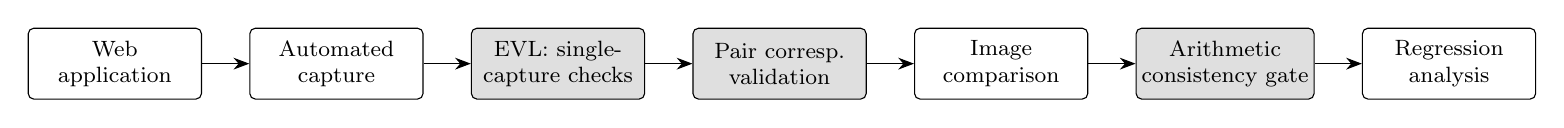
\begin{tikzpicture}[font=\footnotesize,
 box/.style={draw,rounded corners=2pt,minimum height=9mm,minimum width=22mm,align=center,inner sep=2pt},
 ev/.style={box,fill=gray!25,draw=black},
 >={Stealth[length=2mm]}]
\node[box] (a) {Web\\application};
\node[box,right=6mm of a] (b) {Automated\\capture};
\node[ev,right=6mm of b] (c) {EVL: single-\\capture checks};
\node[ev,right=6mm of c] (d) {Pair corresp.\\validation};
\node[box,right=6mm of d] (e) {Image\\comparison};
\node[ev,right=6mm of e] (f) {Arithmetic\\consistency gate};
\node[box,right=6mm of f] (g) {Regression\\analysis};
\foreach \x/\y in {a/b,b/c,c/d,d/e,e/f,f/g}{\draw[->] (\x)--(\y);}
\end{tikzpicture}
\caption{Evidence-validation pipeline. Shaded boxes are validation stages inserted into the conventional capture/compare/decide pipeline. The arithmetic gate necessarily runs after comparison, because it validates the comparison record itself.}
\label{fig:pipeline}
\end{figure*}

\section{Evidence-Validation Framework}\label{sec:framework}
\textit{Placement.} Fig.~\ref{fig:pipeline} places the EVL in a conventional pipeline. Single-capture checks run immediately after capture; pair-level checks (correspondence, membership) run once both captures exist. Both run strictly before the diff back-end. The arithmetic gate validates the comparison record, so it runs after Image Comparison and strictly before Regression Analysis: no threshold decision ever consumes an unvalidated record.

\begin{table}[!t]
\caption{Evidence-Integrity Failure Taxonomy}
\label{tab:taxonomy}
\centering\footnotesize
\begin{tabular}{@{}llp{4.6cm}@{}}
\toprule
ID & Failure class & Description\\
\midrule
F1 & Missing / unreadable & File absent, zero-length, or fails to decode.\\
F2 & Truncated / pre-render & Captured before layout completed; frame incomplete.\\
F3 & Unstable geometry & Dimensions differ beyond what content explains.\\
F4 & File-size anomaly & Size extreme vs.\ session distribution (e.g., blank).\\
F5 & Pair mismatch & $R$ and $C$ depict different logical pages.\\
F6 & Colliding filenames & Filename $\neq$ page identity; collisions mask F5.\\
F7 & Missing membership & Page present in one crawl session only.\\
F8 & Impossible record & $\Dr>\Dw$ for the comparison record.\\
F9 & Abnormal metadata & Load time, viewport, or browser out of range.\\
\bottomrule
\end{tabular}
\end{table}

\textit{Taxonomy and checks.} Table~\ref{tab:taxonomy} lists the nine failure classes and Table~\ref{tab:checks} maps each check to the classes it targets. Only the blank/truncation and arithmetic checks decode pixels. For a pair with heights $h_R,h_C$ and file sizes $s_R,s_C$, let $h_{\mathrm{ratio}}=\max(h_R,h_C)/\min(h_R,h_C)$ and $s_{\mathrm{ratio}}=\max(s_R,s_C)/\min(s_R,s_C)$. The geometry signal (H) fires when $h_{\mathrm{ratio}}\ge\tau_H$, the file-size signal (S) when $s_{\mathrm{ratio}}\ge\tau_S$, and the blank signal (B) when $\min(s_R,s_C)<\tau_B$. The pilot uses one fixed setting for every subject: $\tau_H=2$, $\tau_S=5$ and $\tau_B=50$~KB. These values were fixed before the analysis ($\tau_B$ is carried over from the earlier weather-portal deployment) and were not tuned on the pilot's outcomes; Section~\ref{sec:sens} shows that the results do not depend on them. The timing signal (T) fires when a load time exceeds its session's upper Tukey fence, $Q_3+1.5\,\mathrm{IQR}$.

\begin{table}[!t]
\caption{Validation Checks and Required Inputs}
\label{tab:checks}
\centering\footnotesize
\begin{tabular}{@{}p{2.25cm}p{0.9cm}p{3.35cm}c@{}}
\toprule
Check & Targets & Required input & Pixels?\\
\midrule
Existence / readability & F1 & filesystem entry, manifest record & No\\
Rendering completion & F2, F9 & load time, session load-time distribution & No\\
Geometry ($h_{\mathrm{ratio}}$, $w$-ratio) & F3 & image dimensions (header only) & No\\
File integrity ($s_{\mathrm{ratio}}$, blank) & F4 & file size & No\\
Blank / truncated pixels & F2, F4 & decoded image & Yes\\
Pair correspondence & F5, F6 & normalized URL, manifest filenames & No\\
Missing membership & F7 & both sessions' manifests & No\\
Arithmetic consistency & F8 & record, recomputed $\Dw$ & Yes\\
\bottomrule
\end{tabular}
\end{table}

Two captures correspond only if a normalized page identifier matches (the URL with its fragment and trailing slash removed), not filename equality, since crawlers can collide filenames (F6) while URLs legitimately drift. A page present in only one manifest yields no pair (F7), reported separately from invalid pairs because it affects coverage rather than correctness. $\Dw$ is computed by an independent reimplementation sharing no code with any back-end under test, so a shared bug cannot both produce and validate an error. A pair is \textsc{Invalid} when at least two of H, S, B, T fire, or when the arithmetic check fails (a deterministic rejection, since $\Dr>\Dw$ admits no ambiguity). Algorithm~\ref{alg:sev} gives the procedure.

\begin{algorithm}[!t]
\caption{Screenshot Evidence Validation (SEV)}\label{alg:sev}
\footnotesize
\begin{algorithmic}[1]
\REQUIRE Manifests $M_R,M_C$; capture files; back-end $\mathrm{cmp}(\cdot,\cdot)$
\ENSURE Per page $p$: \textsc{Valid}, \textsc{Invalid}(reasons), or \textsc{NoPair}
\FOR{$p\in \mathrm{keys}(M_R)\cup\mathrm{keys}(M_C)$}
 \IF{$p\notin\mathrm{keys}(M_R)$ \OR $p\notin\mathrm{keys}(M_C)$}
  \STATE emit \textsc{NoPair}($p$); \textbf{continue} \hfill $\triangleright$ F7
 \ENDIF
 \STATE $R_p,C_p\leftarrow \mathrm{load}(M_R[p]),\mathrm{load}(M_C[p])$
 \IF{not readable($R_p$) \OR not readable($C_p$)}
  \STATE emit \textsc{Invalid}($p$,F1); \textbf{continue}
 \ENDIF
 \IF{$\mathrm{norm}(M_R[p].\mathrm{url})\neq \mathrm{norm}(M_C[p].\mathrm{url})$}
  \STATE emit \textsc{Invalid}($p$,F5/F6); \textbf{continue}
 \ENDIF
 \STATE $G\leftarrow\{$H: $h_{\mathrm{ratio}}\!\ge\!\tau_H$, S: $s_{\mathrm{ratio}}\!\ge\!\tau_S$, B: $\min(s_R,s_C)\!<\!\tau_B$, T: $\max(\ell_R,\ell_C)\!>\!\mathrm{fence}\}$
 \IF{$|G|\ge 2$}
  \STATE emit \textsc{Invalid}($p$,$G$); \textbf{continue} \hfill $\triangleright$ F2/F3/F4/F9
 \ENDIF
 \STATE $\Dr\leftarrow \mathrm{cmp}(R_p,C_p).\mathrm{changed}$
 \STATE $\Dw\leftarrow \mathrm{countUnequal}(\mathrm{align}(R_p,C_p))$
 \IF{$\Dr>\Dw$}
  \STATE emit \textsc{Invalid}($p$,F8); \textbf{continue}
 \ENDIF
 \STATE emit \textsc{Valid}($p$)
\ENDFOR
\end{algorithmic}
\end{algorithm}

\section{Study Design}
\subsection{Methodological framework}
The study proceeds in four phases (Fig.~\ref{fig:method}). \emph{Phase~1} builds the capture archive: a crawler visits each subject in repeated sessions and writes a screenshot and a dated manifest per page. \emph{Phase~2} pairs captures across sessions by normalized page identifier and applies the metadata-tier checks (existence, geometry, file size, timing, correspondence, membership). \emph{Phase~3} runs the pre-existing diff back-end on the surviving pairs, recomputes $\Dw$ independently, and applies the arithmetic gate. \emph{Phase~4} computes the metrics below, with confidence intervals, and the wall-clock cost of each check tier. Failure classes F1--F9 are assigned in Phases~2 and~3.

\begin{figure}[!t]
\centering
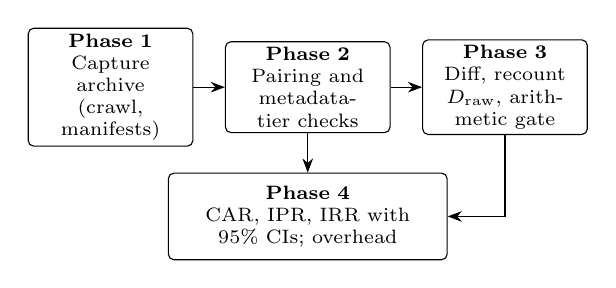
\begin{tikzpicture}[font=\scriptsize,
 box/.style={draw,rounded corners=2pt,text width=1.95cm,minimum height=11mm,align=center,inner sep=2pt},
 >={Stealth[length=1.8mm]}]
\node[box] (p1) {\textbf{Phase 1}\\Capture archive\\(crawl, manifests)};
\node[box,right=4mm of p1] (p2) {\textbf{Phase 2}\\Pairing and metadata-tier checks};
\node[box,right=4mm of p2] (p3) {\textbf{Phase 3}\\Diff, recount $\Dw$, arithmetic gate};
\node[box,below=5mm of p2,text width=3.4cm] (p4) {\textbf{Phase 4}\\CAR, IPR, IRR with 95\% CIs; overhead};
\draw[->] (p1)--(p2); \draw[->] (p2)--(p3); \draw[->] (p3.south)|-(p4.east); \draw[->] (p2)--(p4);
\end{tikzpicture}
\caption{Methodological framework of the pilot study.}
\label{fig:method}
\end{figure}

\textit{Research questions.} This pilot answers three questions that need no ground-truth labels. \textbf{RQ1:} How often do automated screenshot pipelines produce potentially invalid evidence, measured as capture anomaly rate (CAR) and invalid pair rate (IPR)? \textbf{RQ2:} How effectively does normalized-URL/page-ID correspondence prevent mismatched comparisons relative to filename pairing? \textbf{RQ3:} Can the arithmetic check detect impossible records independently of labels and of the comparison algorithm, measured by the impossible record rate (IRR)? Per-class detection quality and precision/recall against a blinded human audit are left to future work (Section~\ref{sec:disc}).

\textit{Harness and comparison records.} We extend the crawler and capture-archive components of a previously deployed harness~\cite{avqrepo}. No subject, session, capture date, or measurement is shared with that earlier deployment, whose corpus is one weather and news portal crawled in November 2025. New here are (i) a metadata schema with normalized page identifiers and manifest membership, (ii) an independent raw-pixel-inequality counter, and (iii) the pilot below. A headless Chromium crawler driven by Puppeteer~\cite{puppeteer} performs a breadth-first, in-domain crawl and captures a full-page PNG per page at a fixed viewport width; each session writes a dated manifest (URL, depth, screenshot path, load time, timestamp), from which, with the files, we derive normalized URLs, dimensions and file sizes. The comparison records were produced by the repository's own diff back-end, retained unmodified. It reads the two PNGs of a page, crops both to the smaller common size if their dimensions differ, and calls pixelmatch~\cite{pixelmatch} (colour-distance threshold 0.1, anti-aliased pixels counted as changed), then stores the changed-pixel count. It was run once per subject after all crawls had finished and before this analysis began, so we treat its output as an independently produced record and check it after the fact rather than generating it ourselves. Following the archive's pairing, we attribute each subject's records to its first two sessions; Section~\ref{sec:root} tests that attribution.

\textit{Subjects and sessions.} Seven documentation/reference sites (nodejs.org, developer.mozilla.org, docs.github.com, en.wikipedia.org, python.org, w3.org, web.dev) were crawled on 2026-08-30 at a 1366~px viewport, depth 3, 20 URLs per session, with 2--3 sessions per subject about 10--20 minutes apart.

\textit{Metrics.} We report
\begin{align}
\mathrm{CAR}&=\frac{\#\text{anomalous captures}}{\#\text{total captures}},\\
\mathrm{IPR}&=\frac{\#\text{invalid pairs}}{\#\text{all comparison pairs}},\\
\mathrm{IRR}&=\frac{\#\text{arithmetically impossible records}}{\#\text{all comparison records}},
\end{align}
each with a 95\% Wilson score interval, plus wall-clock overhead per pair for the metadata-only and pixel-reading checks. Because captures within a session share a crawler run, the CAR interval treats entries as independent and is therefore, if anything, optimistic. All analysis scripts are publicly released at \url{https://github.com/Tanveerrifu/AutoVisQA}.

\section{Results}
\subsection{Whole-subject failures}
Two of seven subjects (28.6\%) yielded no comparable pairs. The w3.org crawl reached only its seed URL (1 of 20) and was never re-crawled, a subject-level instance of F7; the web.dev crawl produced zero screenshots and no manifest (F1). Neither failure is visible from the surviving subjects' diff reports, so reporting only subjects that produced pairs would understate how often evidence-integrity failures occur.

\begin{table}[!t]
\caption{Within-Session Filename-Collision Rate (CAR)}
\label{tab:car}
\centering\footnotesize
\begin{tabular}{@{}lcccc@{}}
\toprule
Subject & Sess.~1 & Sess.~2 & Sess.~3 & Affected\\
\midrule
Python & 8/20 & 4/20 & 0/20 & 12/60\\
Wikipedia & 9/20 & 2/20 & 0/20 & 11/60\\
GitHub Docs & 5/20 & 2/20 & 0/20 & 7/60\\
MDN & 3/20 & 0/20 & -- & 3/40\\
nodejs & 2/20 & 0/20 & -- & 2/40\\
\midrule
Total & \multicolumn{3}{c}{} & 35/260 (13.5\%)\\
\bottomrule
\end{tabular}
\end{table}

\subsection{Capture-level anomalies (RQ1)}
Across the five paired subjects' 13 session-crawls, 260 manifest entries were logged. Of these, 35 (CAR = 13.5\%, 95\% CI 9.8--18.1\%) share an on-disk filename with another entry from the same session: the crawler derives filenames from URLs without fully handling fragment identifiers, so distinct URLs (e.g., \texttt{python.org/}, \texttt{python.org/\#top}, \texttt{python.org/\#site-map}) silently overwrite one file. Collisions fell across each subject's same-day sessions (Python: 8, 4, 0; Table~\ref{tab:car}), consistent with the crawler's filename logic being corrected between runs rather than a static tool property.

\subsection{Invalid pairs and pair correspondence (RQ1, RQ2)}
Matching first- and second-session pages by normalized URL gave 81 pairs; 16 further URLs appeared in only one manifest (F7). Of the 81 pairs, 8 (9.9\%) are tainted by a within-session filename collision (F6). Filename correspondence alone catches none of these, since a tainted \texttt{home.png} is indistinguishable from a clean one to a filename matcher; only cross-checking manifests for duplicate basenames exposes the taint (RQ2). Of the 73 untainted pairs, one (Wikipedia's \texttt{Special:Random}) fires both geometry ($h_{\mathrm{ratio}}=15.3\times$) and file-size ($s_{\mathrm{ratio}}=18.5\times$) signals and is withheld: its URL matches exactly, but it redirects to a different article on every visit. URL correspondence cannot catch this by design, but the geometry check does, so the checks act as partially redundant safety nets. In total 9 of 81 pairs are invalid (IPR = 11.1\%, 95\% CI 6.0--19.8\%; Table~\ref{tab:subject}).

\begin{table}[!t]
\caption{Pilot Corpus and Validation Outcomes by Subject (First- vs.\ Second-Session Comparison)}
\label{tab:subject}
\centering\footnotesize
\begin{tabular}{@{}lccccc@{}}
\toprule
Subject & $n$ & F6 tainted & Geom.\ invalid & Reached arith.\ & Impossible (F8)\\
\midrule
Python & 14 & 2 & 0 & 12 & 1\\
nodejs & 19 & 1 & 0 & 18 & 0\\
MDN & 18 & 1 & 0 & 17 & 0\\
Wikipedia & 13 & 2 & 1 & 10 & 2\\
GitHub Docs & 17 & 2 & 0 & 15 & 0\\
\midrule
Total & 81 & 8 & 1 & 72 & 3\\
\bottomrule
\end{tabular}
\end{table}

\begin{figure*}[!t]
\centering
\begin{tabular}{@{}cc@{}}
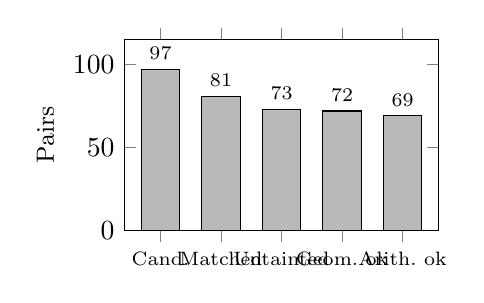
\begin{tikzpicture}
\begin{axis}[ybar,width=0.46\textwidth,height=4.0cm,bar width=14pt,ymin=0,ymax=115,
 ylabel={Pairs},symbolic x coords={Cand.,Matched,Untainted,Geom.\ ok,Arith.\ ok},xtick=data,
 x tick label style={font=\scriptsize},nodes near coords,nodes near coords style={font=\scriptsize},
 every axis label/.append style={font=\small},enlarge x limits=0.15]
\addplot[fill=gray!55] coordinates {(Cand.,97) (Matched,81) (Untainted,73) (Geom.\ ok,72) (Arith.\ ok,69)};
\end{axis}
\end{tikzpicture}
&
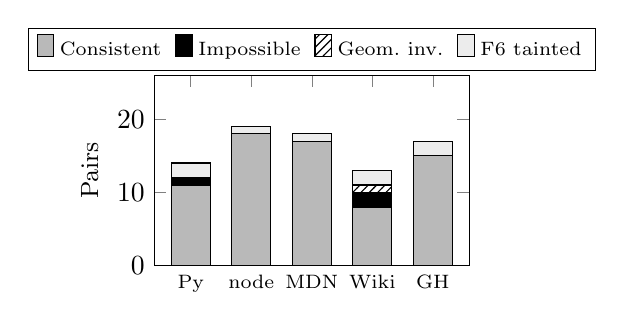
\begin{tikzpicture}
\begin{axis}[ybar stacked,width=0.46\textwidth,height=4.0cm,bar width=14pt,ymin=0,ymax=26,
 ylabel={Pairs},symbolic x coords={Py,node,MDN,Wiki,GH},xtick=data,
 x tick label style={font=\scriptsize},legend style={font=\scriptsize,at={(0.5,1.02)},anchor=south,legend columns=4,/tikz/every even column/.append style={column sep=3pt}},
 every axis label/.append style={font=\small},enlarge x limits=0.15]
\addplot[fill=gray!55] coordinates {(Py,11)(node,18)(MDN,17)(Wiki,8)(GH,15)};
\addplot[fill=black] coordinates {(Py,1)(node,0)(MDN,0)(Wiki,2)(GH,0)};
\addplot[fill=white,postaction={pattern=north east lines}] coordinates {(Py,0)(node,0)(MDN,0)(Wiki,1)(GH,0)};
\addplot[fill=gray!15] coordinates {(Py,2)(node,1)(MDN,1)(Wiki,2)(GH,2)};
\legend{Consistent,Impossible,Geom.\ inv.,F6 tainted}
\end{axis}
\end{tikzpicture}\\
\small (a) Pairs surviving each gate & \small (b) Outcomes by subject
\end{tabular}
\caption{Pilot data. (a) Candidate URL-slots (97) surviving each gate: matched by normalized URL (81; 16 dropped as F7), untainted by F6 (73), passed geometry/file-size/timing (72), and arithmetically consistent (69). (b) Per-subject outcomes.}
\label{fig:pilot}
\end{figure*}

\subsection{Arithmetic consistency (RQ3)}
Each of the 72 pairs passing upstream validation was checked against the back-end's pre-existing record by recomputing $\Dw$. Three (IRR = 3/72 = 4.2\%, 95\% CI 1.4--11.5\%) are impossible:
\begin{itemize}
\item Wikipedia, \texttt{Special:RecentChanges}: reported 12.902\% vs.\ recomputed 0.0\%. The attached captures are byte-identical (797,441 bytes each), so no definition of ``changed pixels'' can be nonzero for them.
\item Wikipedia, \texttt{Special:Search}: reported 0.001\% vs.\ 0.0\%, again from byte-identical inputs (64,922 bytes).
\item Python, \texttt{about/apps}: reported 0.068\% vs.\ 0.0203\% (2,849 vs.\ 849 pixels on a 1366$\times$3062 capture).
\end{itemize}
All three remain impossible under a lenient 30-level per-channel tolerance, ruling out anti-aliasing. Two further violations occur among pairs already withheld as F6-tainted (Python \texttt{home.png}: 19.866\% vs.\ 0.089\%; \texttt{about.png}: 0.055\% vs.\ 0.0\%); without the upstream gates they would masquerade as diff-algorithm bugs, and IRR would be 5/81 = 6.2\% (95\% CI 2.7--13.6\%).



\subsection{Metadata-only vs.\ pixel-level validation, and overhead}
The metadata-only tier (correspondence, geometry, file size, timing) catches all 9 invalid pairs without decoding a pixel, but zero of the 3 impossible records, which by construction passed every metadata signal. Only the pixel tier catches them. The tiers thus catch disjoint problems, and only together flag all 12 of 81 problematic pairs (14.8\%, 95\% CI 8.7--24.1\%). On the analysis machine, the metadata tier processed all 81 pairs in 0.21 s (2.6 ms/pair); adding the pixel tier (blank/truncation decode plus raw recount) over all 114 pairs reaching it across every session-pair took 26.4 s (232 ms/pair), about $89\times$ costlier. Fig.~\ref{fig:pilot} summarizes how pairs are removed at each gate.

\subsection{Ground truth for the impossible records}\label{sec:root}
To check the F8 verdicts against ground truth rather than against another heuristic, we re-executed the archive's back-end (pixelmatch 5.3.0, same settings) on every session pair of every subject and matched its output to each stored record. Every flagged record is reproduced exactly, and every one is a genuine pipeline defect. For the three subjects crawled three times, the back-end had compared the \emph{second and third} sessions, not the first and second to which the archive attributes the records; the three gated violations are of this kind (e.g., \texttt{about/apps}: 2,849 changed pixels between sessions 2 and 3, against 194 between sessions 1 and 2). The two F6-tainted violations come from a collision \emph{inside} the diff tool: its filename normalization strips a numeric suffix, so the third session's \texttt{about\_2.png} and \texttt{home\_2.png} were compared in place of \texttt{about.png} and \texttt{home.png}. Re-attached to the pairs they actually describe, all 93 stored records satisfy $\Dr\le\Dw$. The invariant thus raised no false alarm (5 of 5 verified), but it is one-sided: 17 of the 81 records describe a different capture pair from the one they are attached to, and it flagged the 5 whose reported count exceeded the attached pair's raw count (29\%). Every defect it exposed lay in the plumbing around the diff algorithm, not in the algorithm.

\subsection{Independent confirmation and sensitivity}\label{sec:sens}
\textit{Recount with an established tool.} We recounted $\Dw$ on all 72 pairs with ImageMagick~\cite{imagemagick} 6.9 (\texttt{compare -metric AE -fuzz 0\%}, applied in horizontal bands because of its image-height limit). The counts agree exactly with our reimplementation on 71 pairs and differ by one pixel (1{,}130{,}646 vs.\ 1{,}130{,}647 of about 6.9 million) on the other. All three impossible records are confirmed (849, 0 and 0 raw-unequal pixels), and the two attached Wikipedia captures have identical SHA-256 digests.

\textit{Threshold sensitivity.} Re-running the metadata tier for $\tau_H\in\{1.25,1.5,2,3,5,10\}$ and $\tau_S\in\{2,3,5,10,15\}$ leaves the invalid-pair count at 9 in every one of the 30 settings, because the single geometry-invalid pair exceeds all of them ($h_{\mathrm{ratio}}=15.3\times$, $s_{\mathrm{ratio}}=18.5\times$) and the F6 verdicts do not use thresholds.

\section{Discussion and Limitations}\label{sec:disc}
Invalid evidence is dangerous because it is silent: a crash halts a pipeline, but a truncated or mispaired screenshot yields a plausible number a threshold acts on. Two of our three impossible records were attached to byte-identical inputs, where no difference could exist, yet the report showed one with no signal marking it suspect. The pre-render capture of Section~I shows the worst case: invalid evidence was not merely tolerated but ranked among the largest regressions, inserting a spurious high-confidence signal rather than a low-confidence one an engineer might discount.

A better diff algorithm cannot fix invalid input: SSIM, LPIPS, or a learned metric would compute a more precise answer to the wrong question. Validity and perceptual accuracy are orthogonal, which is why the EVL sits before differencing rather than acting as another metric.

\textit{Errors are asymmetric.} The EVL excludes a comparison rather than adjudicating it. A false withhold removes an informative comparison and should be logged; driving missed invalid pairs to zero would raise false withholds, a tradeoff only an audited study can expose.

\textit{Practical guidance.} (1) Insert validation as a distinct, logged stage; every check in Table~\ref{tab:checks} works on output an existing back-end already produces. (2) Start from conservative thresholds such as ours and calibrate $\tau_H,\tau_S,\tau_B$ and the timing fence per application from its own capture history. (3) Treat \textsc{Invalid} as excluded from the decision and surface it for re-capture, never silently dropped. (4) Run the cheap metadata tier on every pre-merge comparison and the pixel tier in nightly or release-candidate gates; since the tiers catch disjoint failures, neither substitutes for the other. (5) Store the content hashes of both captures in every comparison record; misattribution then becomes checkable exactly, closing the gap left by the one-sided invariant.

\textit{Threats to validity.} \emph{Internal:} rates are conditional on the fixed thresholds of Section~\ref{sec:framework}, which were set before computing CAR/IPR/IRR and are not tuned post hoc; the sensitivity check above shows they do not change IPR. Most verdicts need no subjective judgment: F6 follows from duplicate filenames in the manifests, F8 from recomputation and is confirmed by re-executing the back-end (Section~\ref{sec:root}), and only the single geometry verdict (a page that redirects to a different article) rests on inspection. Even so, without a blinded human audit, ambiguous cases (a legitimately grown page vs.\ a truncated one) could be misclassified, and pages that pass every check yet change on every load (e.g., live timestamps) are out of scope. Apart from F8, whose precision is established by reproduction, detection accuracy is therefore not measured. \emph{Construct:} ``validity'' is operationalized as the checks in Table~\ref{tab:checks}; passing them does not prove a pair trustworthy in every sense. The arithmetic check is exempt from this concern, since $\Dr\le\Dw$ is a mathematical property. \emph{External:} the pilot covers five documentation sites at one dynamism level, 2--3 sessions each, one browser engine and viewport, and the sample is small (81 pairs), hence the wide intervals above. Our cross-check against ImageMagick covers pixel counting only; we have not compared other diff libraries. The pilot shows these failures occur in a real deployment, not their general rate.

\textit{Future work.} A larger study should span subjects of varying dynamism with at least ten sessions each (roughly 140--250 pairs per subject for a $\pm0.05$ half-width), test further diff libraries, and add a blinded two-rater audit (Cohen's $\kappa$) to measure per-class precision and recall.

\section{Conclusion}
Automated visual regression testing has concentrated its rigor on how to compare two images and treated the validity of those images as an unstated precondition. We gave that precondition a taxonomy, a lightweight validation layer built from information pipelines already produce, and an invariant, $\Dr\le\Dw$, that certifies impossible evidence without labels or dependence on the comparison algorithm. On a real archive, 13.5\% of captures collided on filename, 11.1\% of matched pairs were invalid, and 4.2\% of records reaching the arithmetic gate were impossible, including records attached to byte-identical inputs that metadata checks cannot catch; re-executing the back-end traced every one to a real pipeline defect. ``Validate first, compare second'' is a cheap discipline. The analysis scripts, a reusable EVL tool, and a corrected diff back-end that stores content hashes are released at \url{https://github.com/Tanveerrifu/AutoVisQA}.

\begin{thebibliography}{99}\footnotesize
\bibitem{barr2015} E. T. Barr, M. Harman, P. McMinn, M. Shahbaz, and S. Yoo, ``The oracle problem in software testing: A survey,'' \emph{IEEE Trans. Softw. Eng.}, vol. 41, no. 5, 2015.
\bibitem{parry2022} O. Parry, G. M. Kapfhammer, M. Hilton, and P. McMinn, ``A survey of flaky tests,'' \emph{ACM Trans. Softw. Eng. Methodol.}, vol. 31, no. 1, Art. 17, 2022.
\bibitem{romano2021} A. Romano, Z. Song, S. Grandhi, W. Yang, and W. Wang, ``An empirical analysis of UI-based flaky tests,'' in \emph{Proc. ICSE}, 2021.
\bibitem{pei2026} Y. Pei, J. Sohn, and M. Papadakis, ``An empirical study of web visual flakiness: Characterisation and fix strategies,'' \emph{J. Syst. Softw.}, vol. 237, art. 112826, 2026.
\bibitem{webdiff} S. R. Choudhary, H. Versee, and A. Orso, ``WEBDIFF: Automated identification of cross-browser issues in web applications,'' in \emph{Proc. IEEE ICSM}, 2010.
\bibitem{xpert} S. R. Choudhary, M. R. Prasad, and A. Orso, ``X-PERT: Accurate identification of cross-browser issues in web applications,'' in \emph{Proc. ICSE}, 2013.
\bibitem{redecheck} T. A. Walsh, G. M. Kapfhammer, and P. McMinn, ``ReDeCheck: An automatic layout failure checking tool for responsively designed web pages,'' in \emph{Proc. ACM ISSTA}, 2017.
\bibitem{mahajan2015} S. Mahajan and W. G. J. Halfond, ``Detection and localization of HTML presentation failures using computer vision-based techniques,'' in \emph{Proc. IEEE ICST}, 2015.
\bibitem{pesto} M. Leotta, A. Stocco, F. Ricca, and P. Tonella, ``Pesto: Automated migration of DOM-based web tests towards the visual approach,'' \emph{Softw. Test. Verif. Reliab.}, vol. 28, no. 4, art. e1665, 2018.
\bibitem{stocco2018} A. Stocco, R. Yandrapally, and A. Mesbah, ``Visual web test repair,'' in \emph{Proc. ACM ESEC/FSE}, 2018.
\bibitem{bajammal2018} M. Bajammal and A. Mesbah, ``Web canvas testing through visual inference,'' in \emph{Proc. IEEE ICST}, 2018.
\bibitem{tran2021} H. K. V. Tran, M. Unterkalmsteiner, J. B\"orstler, and N. b. Ali, ``Assessing test artifact quality---A tertiary study,'' \emph{Inf. Softw. Technol.}, vol. 139, art. 106620, 2021.
\bibitem{chen1998} T. Y. Chen, S. C. Cheung, and S. M. Yiu, ``Metamorphic testing: A new approach for generating next test cases,'' HKUST, Tech. Rep. HKUST-CS98-01, 1998.
\bibitem{wang2004} Z. Wang, A. C. Bovik, H. R. Sheikh, and E. P. Simoncelli, ``Image quality assessment: From error visibility to structural similarity,'' \emph{IEEE Trans. Image Process.}, vol. 13, no. 4, 2004.
\bibitem{zhang2018} R. Zhang, P. Isola, A. A. Efros, E. Shechtman, and O. Wang, ``The unreasonable effectiveness of deep features as a perceptual metric,'' in \emph{Proc. IEEE/CVF CVPR}, 2018.
\bibitem{puppeteer} Chrome DevTools Team, ``Puppeteer.'' [Online]. Available: https://pptr.dev
\bibitem{resemble} maurycyg, ``node-resemble.js, Issue \#22,'' 2016. [Online]. Available: https://github.com/lksv/node-resemble.js/issues/22
\bibitem{avqrepo} T. Hasan, ``AutoVisQA: Capture archive and analysis scripts,'' 2026. [Online]. Available: https://github.com/Tanveerrifu/AutoVisQA
\bibitem{pixelmatch} Mapbox, ``pixelmatch.'' [Online]. Available: https://github.com/mapbox/pixelmatch
\bibitem{imagemagick} ImageMagick Studio LLC, ``ImageMagick.'' [Online]. Available: https://imagemagick.org
\end{thebibliography}
\end{document}
